\subsection*{Task 3}

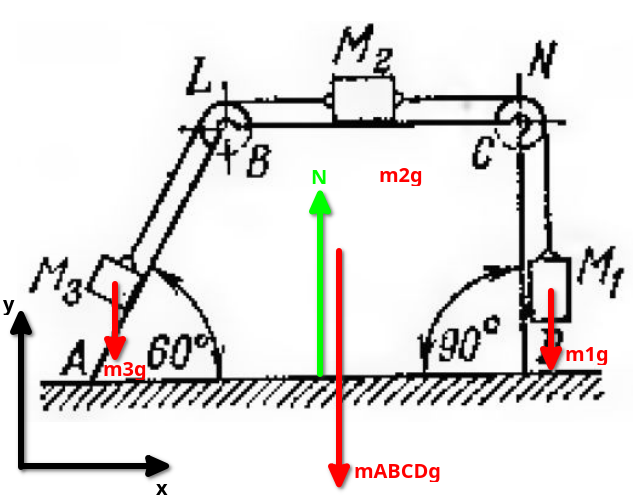
\includegraphics[width=\linewidth]{task3.png}

\begin{enumerate}
    \item I will solve the task as it was supposed by "Meshcherskiy", so mass of $ABCD$ will be 100.
    \item RO - system of 4 bodies, $ABCD$, body 1, body 2, body 3 - translatory motion.
    \item Method: CoM
    \item Conditions: \\
          I will write only for x axis as it is enough to complete this task \\
          \begin{tabular}{|c|c|c|}
              \hline
              $$          & initial & final                       \\
              \hline
              $x_{ABCD}$  & $x_0$   & $x_0 + s$                   \\
              \hline
              $x_{body1}$ & $x_1$   & $x_1 + s$                   \\
              \hline
              $x_{body2}$ & $x_2$   & $x_2 + s + d$               \\
              \hline
              $x_{body3}$ & $x_3$   & $x_3 + s + d \cos(\pi / 3)$ \\
              \hline
              $x'$        & $0$     & $0$                         \\
              \hline
              $x''$       & $0$     & $0$                         \\
              \hline
          \end{tabular}
    \item Forces analysis: $\vec{G}_{ABCD}$,
          $\vec{G}_{body1}$,
          $\vec{G}_{body2}$,
          $\vec{G}_{body3}$,
          $\vec{N}$ (of the whole system)
    \item Solution:
          \begin{enumerate}
              \item Writing this equation for x axis:
                    \begin{align}
                        M x''_c = 0 \\
                        M x'_c = 0  \\
                        M x_c = 0   \\
                    \end{align}
                    Which means that between initial and final position center of mass did not move.
              \item Equation connecting initial and final position:
                    \begin{align}
                        M x^{init}_{c} = M x^{final}_{c}
                    \end{align}
              \item Using CoM:
                    \begin{align}
                        \sum m_i x^{init}_i = \sum m_i x^{final}_i \\
                        m_1 s + m_2 d + m_2 s + m_3 d \cos(\pi / 3) + m_3 s + m_{ABCD} s = 0
                    \end{align}
          \end{enumerate}
\end{enumerate}
\subsection*{Answer:}
\begin{answer}
    \begin{align}
        s = -\frac{4}{29} \notag
    \end{align}
\end{answer}